\documentclass[11pt,a4paper]{article}

\usepackage[margin = 1in]{geometry}
\usepackage{graphicx}
\usepackage{booktabs}
\usepackage{float}
\usepackage{hyperref}
\usepackage{array}

\title{CS5187 Course Project 1\\Image Feature Matching and Outlier Rejection}
\author{}
\date{\today}

\begin{document}

\maketitle

\section{Overview}
This project implements a classical local feature matching pipeline and evaluates it on five challenging scenarios selected from the assignment list. The five scenarios used in this submission are blur, illumination change, perspective change, scale change, and severe clutter. Each experiment contains two input images and one output image that places the inputs side by side and draws only the RANSAC inlier correspondences.

\section{Pipeline Details}
The pipeline is composed of the following stages:
\begin{enumerate}
    \item Read the input images with PIL and convert them to grayscale.
    \item Compute image gradients using Sobel filters.
    \item Detect keypoints with the Harris corner detector and retain local maxima in a $3 \times 3$ neighborhood.
    \item Extract a simplified SIFT-style descriptor from a $16 \times 16$ patch centered at each keypoint. The patch is divided into $4 \times 4$ cells, and each cell contributes an 8-bin orientation histogram, resulting in a 128-dimensional descriptor.
    \item Match descriptors using SSD distance and filter ambiguous matches with Lowe's ratio test.
    \item Estimate a homography with RANSAC and keep only geometrically consistent inlier matches.
    \item Save a visualization image that concatenates the two inputs horizontally and draws the inlier connections after RANSAC.
\end{enumerate}

The main parameter settings are summarized in Table \ref{tab:params}.

\begin{table}[H]
    \centering
    \caption{Pipeline parameters}
    \label{tab:params}
    \begin{tabular}{ll}
        \toprule
        Parameter & Value \\
        \midrule
        Gaussian smoothing $\sigma$ & 1.0 \\
        Harris constant $k$ & 0.04 \\
        Corner threshold & 0.01 \\
        Descriptor patch size & $16 \times 16$ \\
        Orientation bins & 8 \\
        Lowe ratio threshold & 0.75 \\
        RANSAC iterations & 1000 \\
        RANSAC inlier threshold & 5.0 pixels \\
        Transform model & Homography \\
        \bottomrule
    \end{tabular}
\end{table}

\section{Scene Analysis}
Table \ref{tab:summary} summarizes the numerical results on the five selected scenarios.

\begin{table}[H]
    \centering
    \caption{Result summary on selected scenarios}
    \label{tab:summary}
    \begin{tabular}{p{3.1cm}ccc}
        \toprule
        Scenario & Raw matches & Inlier matches & Inlier ratio \\
        \midrule
        Blur & 131 & 72 & 54.96\% \\
        Illumination change & 532 & 458 & 86.09\% \\
        Perspective change & 146 & 57 & 39.04\% \\
        Scale change & 74 & 6 & 8.11\% \\
        Severe clutter & 21 & 8 & 38.10\% \\
        \bottomrule
    \end{tabular}
\end{table}

\subsection{Scenario 1: Blur}
\begin{figure}[H]
    \centering
    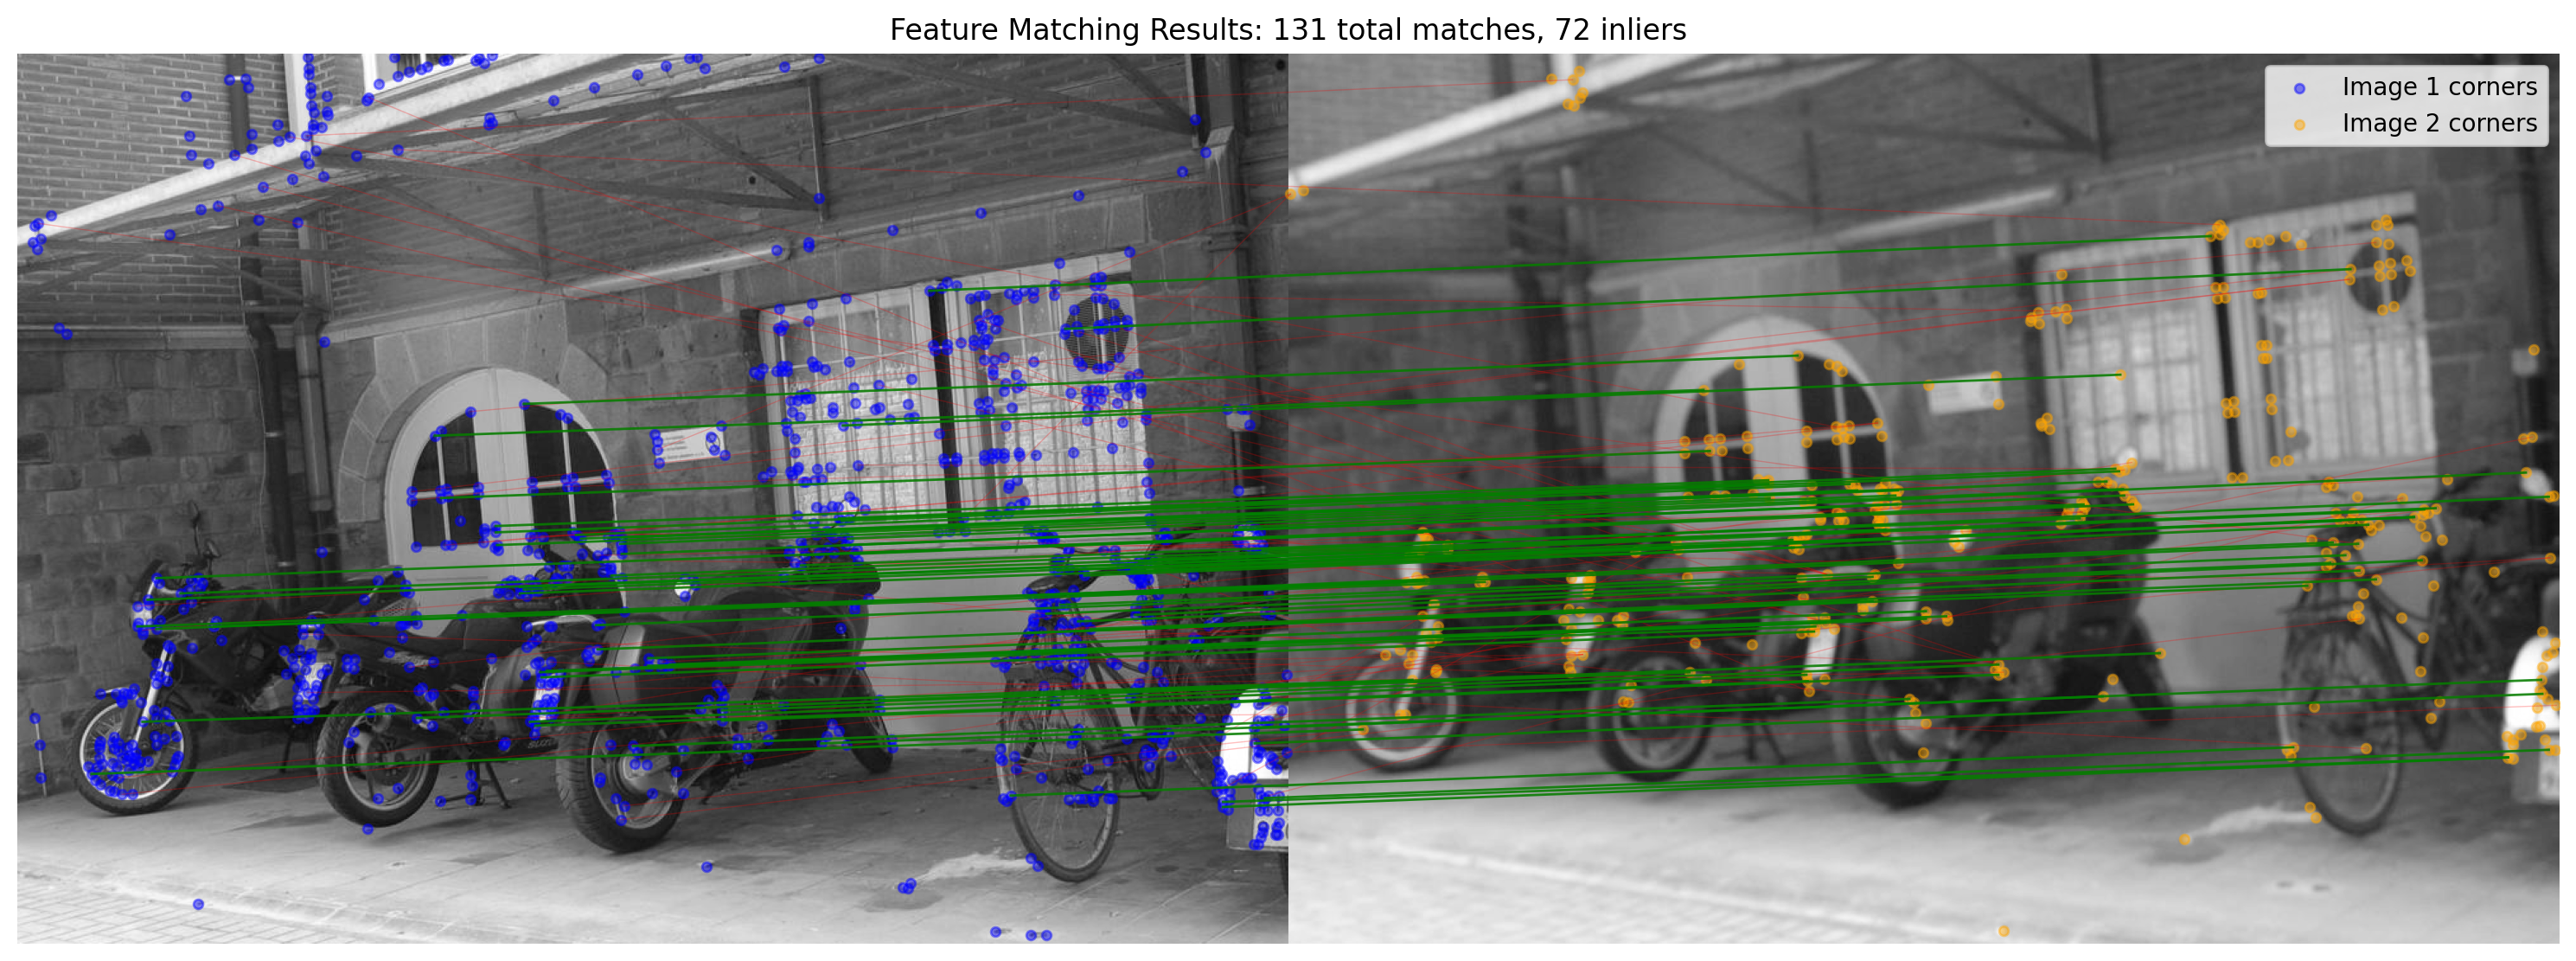
\includegraphics[width = 0.96\textwidth]{../output_images/scenario_01_blur_output.png}
    \caption{Scenario 1: blur / defocus}
\end{figure}

This case is largely successful. Blur suppresses high-frequency image details, so the second image contains fewer strong Harris corners than the first one, but the detector still finds enough stable structural points. The descriptor matching stage produces 131 raw matches, and RANSAC keeps 72 inliers. This indicates that the gradient-histogram descriptor still has moderate robustness under blur. The main degradation happens in the corner detection stage because blur weakens corner responses directly.

\subsection{Scenario 2: Illumination Change}
\begin{figure}[H]
    \centering
    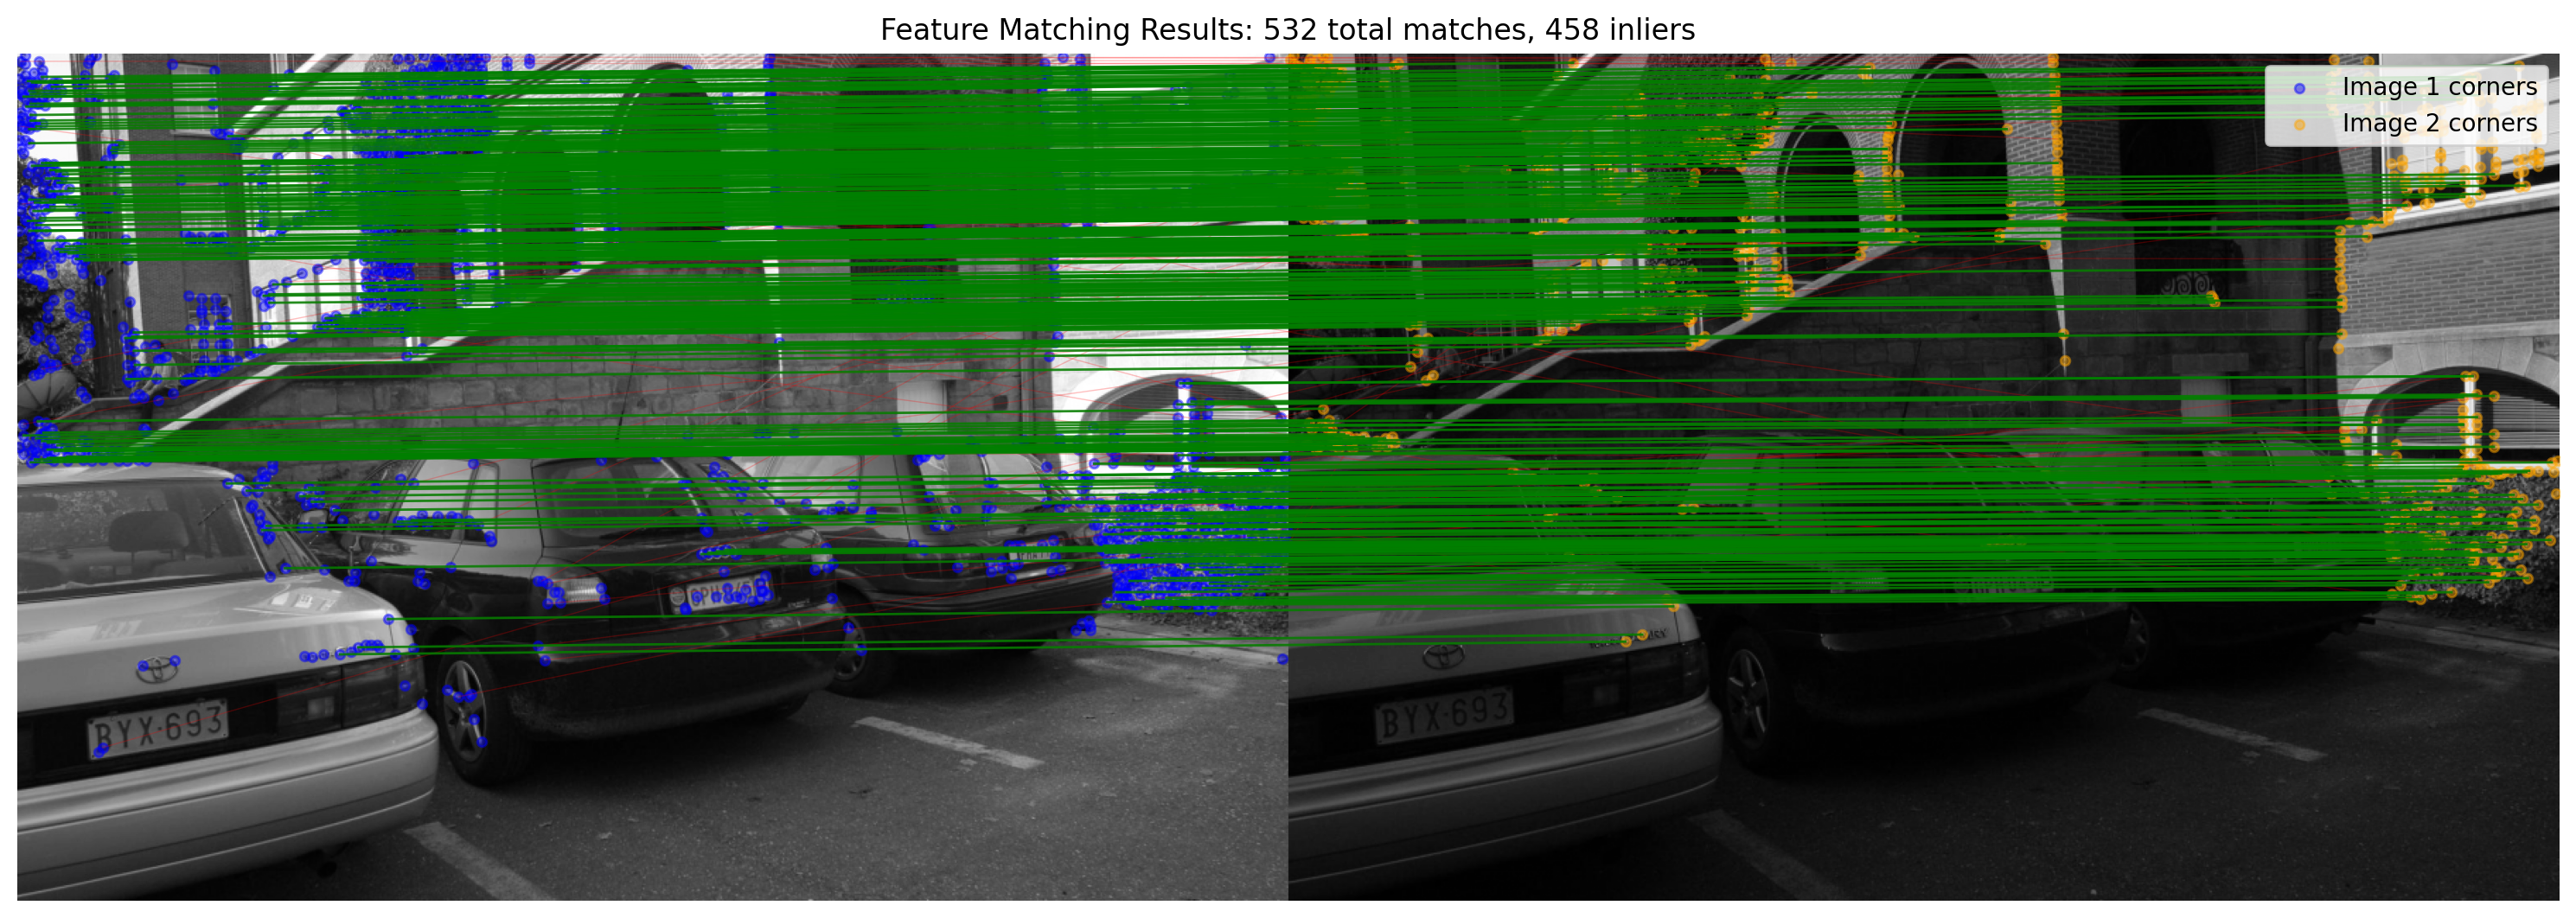
\includegraphics[width = 0.96\textwidth]{../output_images/scenario_02_illumination_output.png}
    \caption{Scenario 2: illumination change}
\end{figure}

This is one of the most successful scenarios. Although the overall brightness changes significantly, the local gradient structure remains similar, so both Harris corners and gradient-based descriptors remain stable. Out of 532 raw matches, 458 survive RANSAC, leading to an inlier ratio above 86\%. This suggests that the current pipeline is fairly robust to moderate illumination variation.

\subsection{Scenario 3: Perspective Change}
\begin{figure}[H]
    \centering
    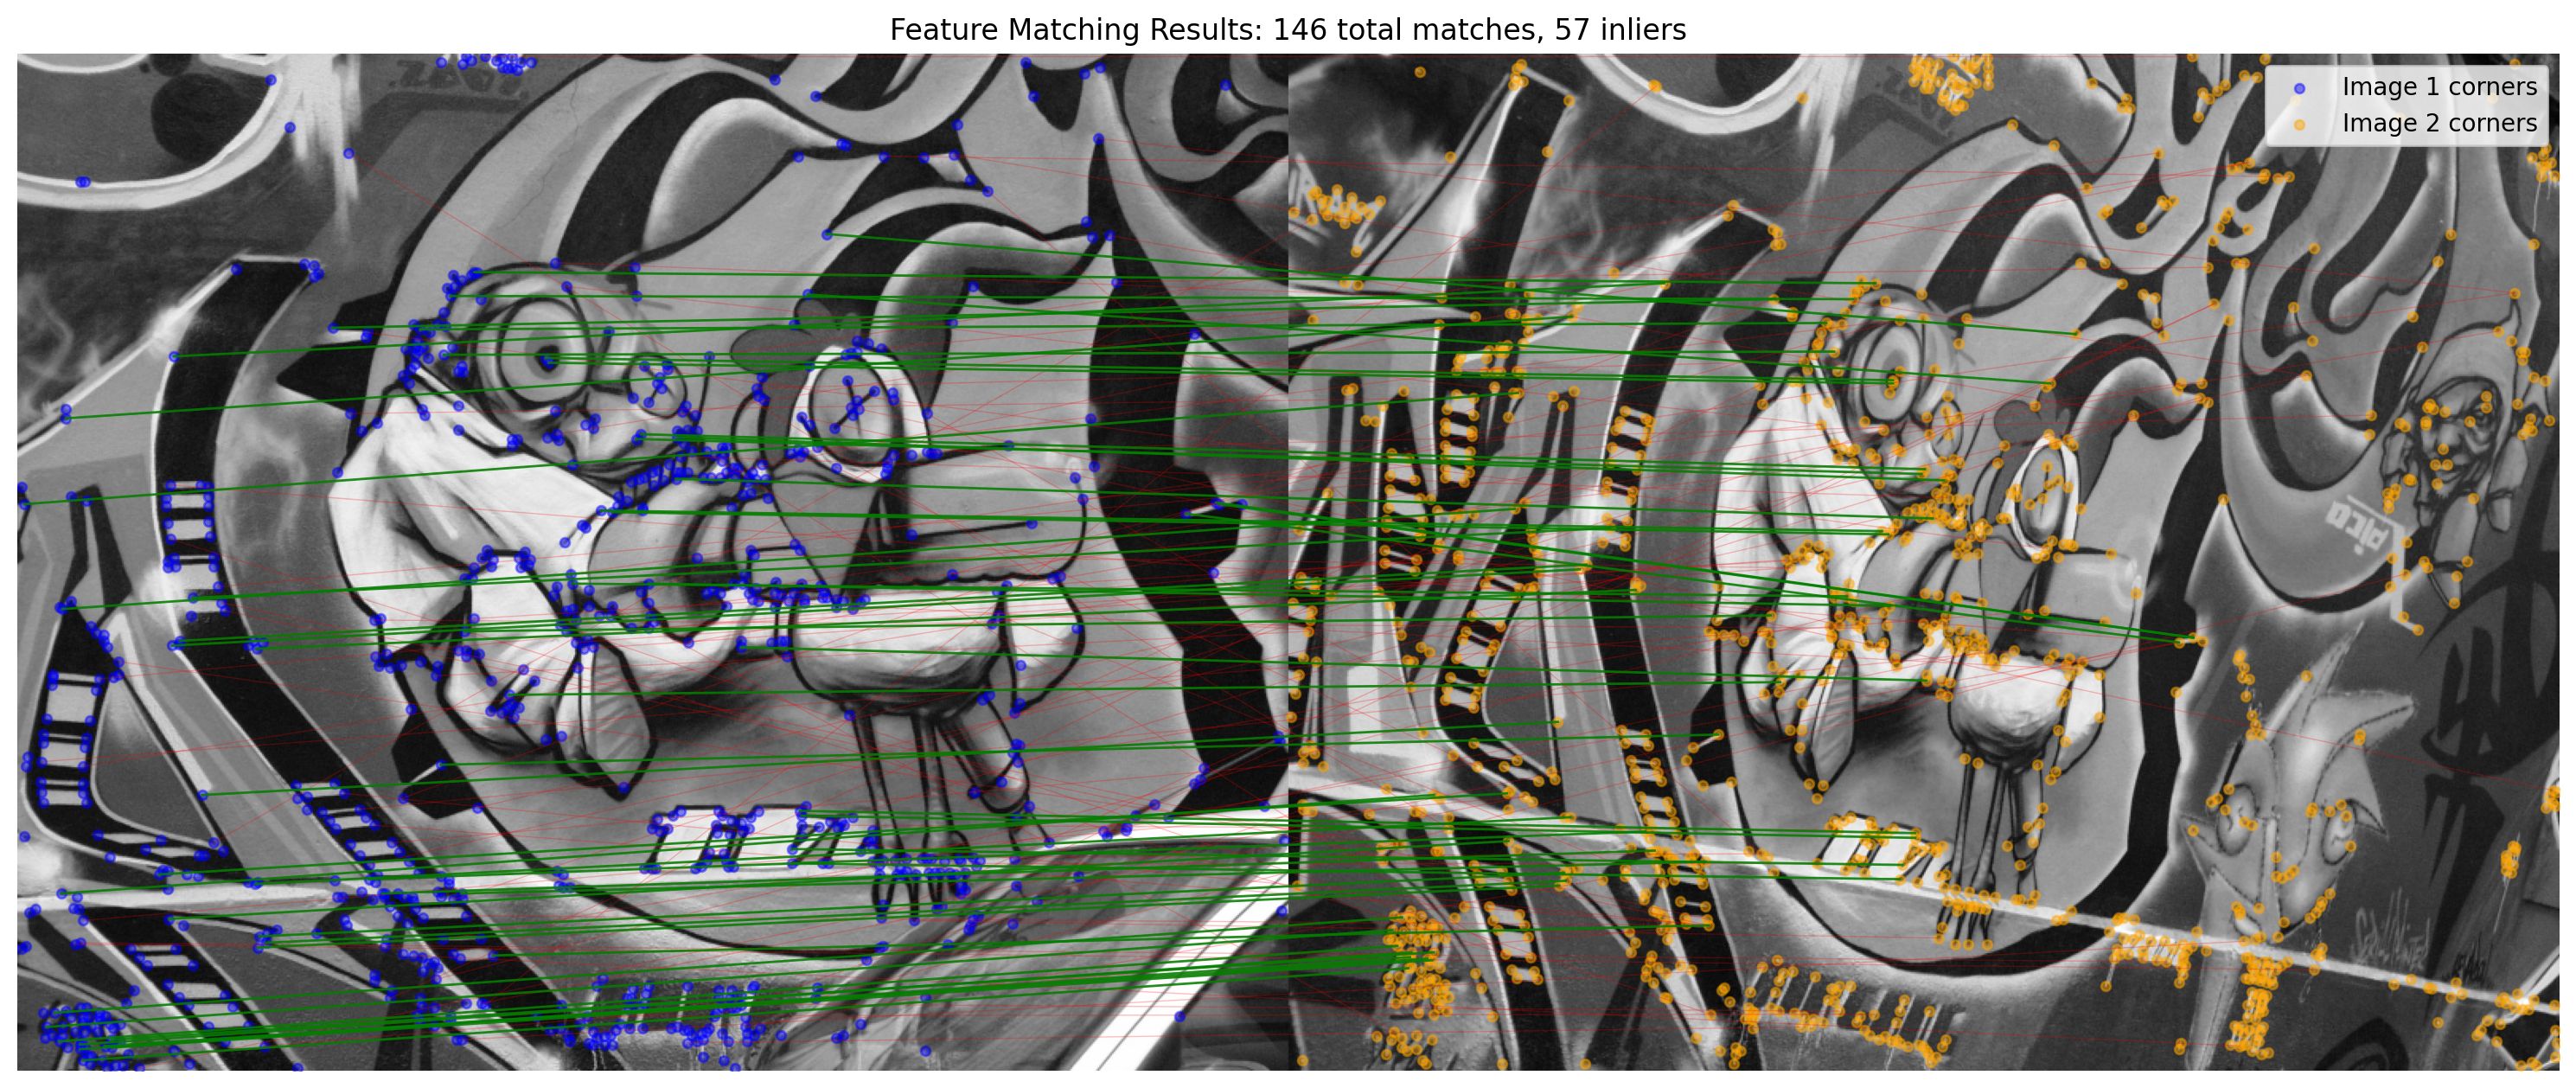
\includegraphics[width = 0.96\textwidth]{../output_images/scenario_03_perspective_output.png}
    \caption{Scenario 3: perspective / viewpoint change}
\end{figure}

This scenario is partially successful. RANSAC retains 57 inliers, which shows that the homography model can absorb a substantial amount of planar viewpoint distortion. However, the inlier ratio is only about 39\%, which means that many incorrect matches are still generated before geometric verification. The main weakness is in the descriptor stage. The current implementation does not perform true scale-space keypoint detection or full orientation alignment, so stronger viewpoint changes reduce descriptor consistency.

\subsection{Scenario 4: Scale Change}
\begin{figure}[H]
    \centering
    \includegraphics[width = 0.96\textwidth]{../output_images/scenario_04_scale_output.png}
    \caption{Scenario 4: scale / zoom}
\end{figure}

This is the weakest scenario in the entire evaluation. Even though Harris detects many corners in both images, the pipeline produces only 74 raw matches and RANSAC keeps only 6 inliers, corresponding to an inlier ratio of about 8\%. The root cause is the lack of true scale invariance. The descriptor mimics the structure of SIFT, but the keypoints are still detected on a single image scale and the local patch size is fixed. Once the object scale changes significantly, the extracted neighborhoods no longer correspond well, and matching quality drops sharply.

\subsection{Scenario 5: Severe Clutter}
\begin{figure}[H]
    \centering
    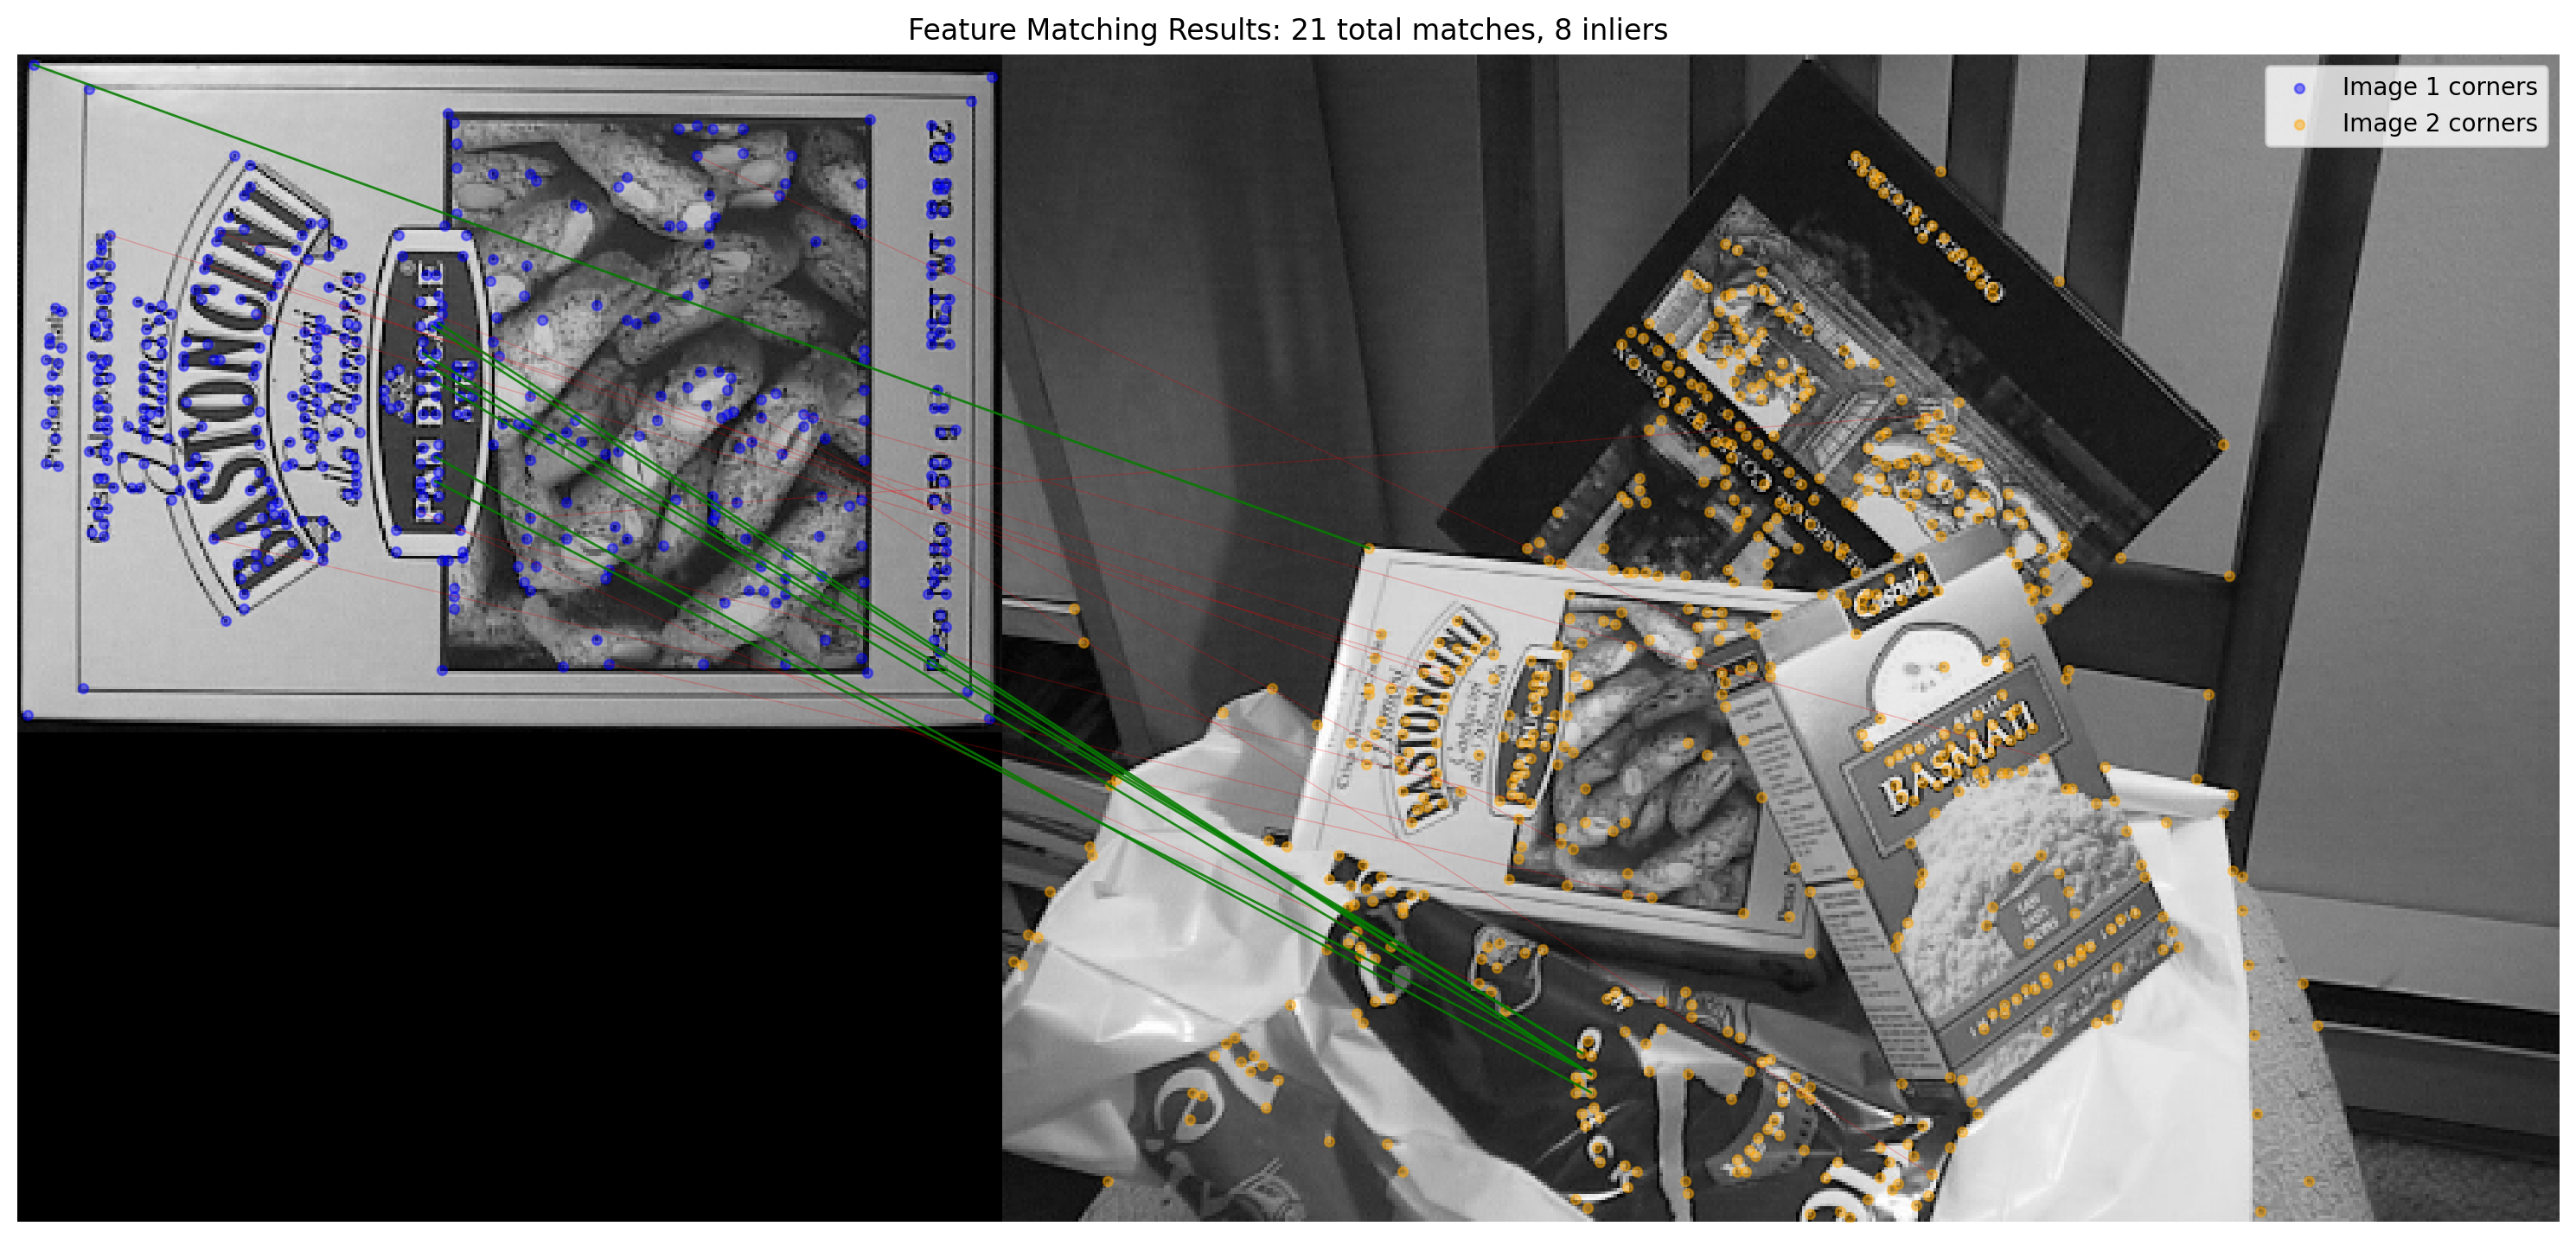
\includegraphics[width = 0.96\textwidth]{../output_images/scenario_05_clutter_output.png}
    \caption{Scenario 5: severe clutter}
\end{figure}

This scenario is difficult but still usable. The second image contains a cluttered background, so Harris detects many irrelevant corners outside the target object. As a result, the descriptor matching stage becomes ambiguous. The pipeline finds only 21 raw matches, but RANSAC is still able to recover 8 geometrically consistent inliers. This means RANSAC plays a critical role in cluttered scenes. The main bottleneck here is not the geometric model but the limited discriminative power of the handcrafted descriptors.

\section{Limitations and Improvements}
The results reveal three main limitations of the current pipeline.

First, the detector does not build a scale space, so the method is very fragile under large scale changes. Harris is not scale invariant by itself, and this is the main reason the scale scenario fails so badly.

Second, although the descriptor uses a gradient-histogram structure, it is still only a simplified approximation of SIFT. Important components of the full SIFT pipeline, such as stable dominant orientation assignment, scale normalization, and more careful histogram interpolation, are missing. Because of that, descriptor distinctiveness is limited under viewpoint changes, blur, and clutter.

Third, the matching stage is relatively basic and relies only on SSD plus Lowe's ratio test. In more ambiguous scenes, this still allows many wrong matches to pass into RANSAC, which then has to clean them up afterward.

If I were to improve the system, I would prioritize the following upgrades:
\begin{itemize}
    \item \textbf{Full SIFT or SURF}: the most direct way to improve robustness to scale and rotation.
    \item \textbf{ORB with BRIEF or BRISK}: a lightweight alternative that still provides more stable keypoint detection and description.
    \item \textbf{Learned local features}, such as SuperPoint + SuperGlue or LoFTR: these methods usually perform much better under illumination change, viewpoint distortion, and clutter.
    \item \textbf{Mutual consistency matching and adaptive thresholds}: these would reduce false matches before RANSAC and improve the quality of geometric estimation.
\end{itemize}

Overall, the current pipeline works well for illumination change and moderate blur, is only moderately reliable under perspective change and clutter, and clearly fails under strong scale variation. This behavior is consistent with what should be expected from a Harris-based handcrafted feature pipeline.

\section{Submission Contents}
The assignment text contains a small inconsistency: Section 3 asks the student to choose 5 out of 10 scenarios, while the deliverable section mentions 10 full scenarios. This submission follows the explicit instruction in Section 3 and therefore contains 5 selected scenarios.

This submission includes:
\begin{itemize}
    \item \texttt{code/}: all main Python source files and runnable batch scripts.
    \item \texttt{input\_images/}: the same 10 renamed input images in folder form.
    \item \texttt{output\_images/}: 5 output images, each containing side-by-side inputs and RANSAC inlier connections.
    \item \texttt{project\_report.tex}: the LaTeX source of this report.
    \item \texttt{project\_report.pdf}: the compiled PDF version of this report.
\end{itemize}

\end{document}
